%%%%%%%%%%%%%%%%%%%%%%%%%%%%%%%%%%%%%%%%%%%%%%%%%%%%%%%%%%%%%%%%%%%%%%%%%%%%%%
%%% REVISED INTRODUCTION STRUCTURE
%%% Current structure has logical gaps: the LLM-in-materials section
%%% interrupts the main narrative flow (problem → methods → gap → our method).
%%%
%%% Current revised order (Round 3 — logical-bridge fix for narrative jump):
%%%   1. Opening: problem statement (adsorption config search matters)
%%%   2. Traditional methods → MLFFs → search-strategy bottleneck → reasoning problem (bridge)
%%%   3. LLM agents as reasoning engines (general → foundational demos → surface science gap)
%%%   4. Adsorb-Agent: first LLM attempt for adsorption search
%%%   5. Limitations of open-loop LLM agents (3 failure modes)
%%%   6. Closing the loop: AdsMind design
%%%   7. Our contribution + negative results
%%%   8. Figure 1: pipeline overview
%%%
%%%%%%%%%%%%%%%%%%%%%%%%%%%%%%%%%%%%%%%%%%%%%%%%%%%%%%%%%%%%%%%%%%%%%%%%%%%%%%


Heterogeneous catalysis underpins the vast majority of industrial chemical processes and is central to emerging clean-energy technologies, including green hydrogen production, CO$_2$ valorization, and sustainable ammonia synthesis~\cite{norskov2004density,greeley2017design}.
In each of these processes, the adsorption of molecular species onto catalyst surfaces---the binding site, orientation, and coordination of the adsorbate---constitutes the critical elementary step that governs activation barriers and reaction selectivity~\cite{norskov2004density}.
Decades of computational catalyst discovery, from descriptor-based screening~\cite{norskov2004density} to high-throughput DFT workflows~\cite{greeley2017design,ulissi2017toward}, have established that accurately identifying the most stable adsorbate--surface configuration is foundational to predicting catalytic performance.
Yet this identification remains a persistent computational bottleneck: the configuration space grows combinatorially, as site types (ontop, bridge, hollow, and their compositional variants), adsorbate orientation, and conformational flexibility combine to produce candidate counts exceeding several hundred for a single intermetallic surface with a polyatomic adsorbate. 

Traditional approaches to adsorption configuration search rely on exhaustive DFT enumeration over canonical site families~\cite{norskov2004density}, genetic algorithms~\cite{vilhelmsen2014genetic}, basin hopping~\cite{wales1997global}, ab initio random structure searching~\cite{pickard2011ab}, and first-passage kinetic Monte Carlo~\cite{reuter2003first}.
These methods require many energy evaluations, each costing hundreds to thousands of CPU-hours, and scale poorly to the complex alloy and multimetallic surfaces of greatest practical interest~\cite{greeley2017design}.
Crucially, these workflows demand substantial expert knowledge to set up and interpret: convergence failures, spin-state sensitivity, and basis-set selection require manual intervention and iterative debugging that cannot be easily automated~\cite{stamatakis2011first}.
As a result, routine adsorption studies on a single surface can consume weeks of specialist time, making high-throughput screening across composition space impractical without large computational teams~\cite{ulissi2017toward}.
This persistent bottleneck has motivated both large-scale benchmark datasets to standardize evaluation and efforts to automate the search strategy itself.
Benchmark datasets such as OC20~\cite{zitnick2020introduction} and OC22~\cite{tran2023oc22} have catalyzed progress by providing standardized evaluation protocols, yet the fundamental search problem remains.

%\subsection{Machine learning surrogates and the remaining search problem}
Fueled by these large-scale benchmark datasets, machine learning force fields (MLFFs) such as MACE/MACE-MP~\cite{batatia2022mace,batatia2023foundation}, CHGNet~\cite{deng2023chgnet}, and EquiformerV2~\cite{liao2023equiformerv2} have dramatically reduced the per-evaluation cost, achieving near-DFT accuracy at orders-of-magnitude speedup.
However, MLFFs solve only the \textit{fast energy evaluation} problem; they do not address the upstream \textit{search strategy} problem of deciding which configurations to evaluate.
Search strategies in computational materials science can be broadly categorized as \textit{open-loop} or \textit{closed-loop}.
In open-loop strategies, the search policy is fixed before evaluation and cannot adapt based on new calculation results.
In closed-loop strategies, each evaluation result feeds back into the search policy, enabling adaptive exploration.
Most current deep-learning-assisted configuration generators---graph neural networks that predict site stability~\cite{reiser2022gnn,gasteiger2022gemnet}, diffusion models that propose crystal structures~\cite{xie2022cdvae,zeni2025mattergen}---remain open-loop: once trained, they cannot adapt based on new calculation results.
This architectural limitation suggests these models cannot recover when their initial proposals miss stable configurations \cite{abolhasani2023rise}, highlighting the need for closed-loop feedback mechanisms that can adapt based on physical evaluation results. 
Large-scale open-loop efforts exemplify both the potential and the ceiling of this paradigm: GNoME~\cite{merchant2023gnome} discovered 2.2~million new crystal structures via GNN-guided screening, yet the pipeline cannot self-correct when its initial guesses miss stable configurations.
Prioritizing candidate configurations among the combinatorially many possibilities requires chemical reasoning---a capability that fixed computational pipelines are ill-suited to provide.

Large language models---which encode broad chemical knowledge and can perform compositional reasoning~\cite{mirza2024chembench,bran2024chemcrow}---have emerged as a natural candidate for this reasoning role.
LLM agents have recently been applied to diverse materials discovery tasks~\cite{zimmermann2025llm,yang2026quasar,stewart2026graphagents,chandrasekhar2026catalyst,weietal2025agentic}, and closed-loop autonomous systems such as A-Lab~\cite{szymanski2023alab} have demonstrated the power of feeding experimental feedback back into the planning loop.
Foundational demonstrations---ChemCrow~\cite{bran2024chemcrow} (tool-augmented LLM for synthesis planning), Coscientist~\cite{boiko2023autonomous} (autonomous chemistry experimentation), and early closed-loop retrosynthesis agents~\cite{schwaller2020predicting}---have established that LLM agents can coordinate multi-step chemical workflows, validating the premise that LLM-driven reasoning can replace manual expert intervention.
While Adsorb-Agent~\cite{ock2026adsorbagent} demonstrates the promise of LLM-driven hypothesis generation, its single-pass architecture employs an LLM planner with EquiformerV2 to generate plausible adsorption hypotheses from natural-language surface descriptions and enumerate configurations, reducing the effective search space relative to naive DFT sweeps.
However, because feedback from physical evaluations is not systematically fed back to the LLM to correct its reasoning, the loop remains open.
Closed-loop agentic systems that couple LLM reasoning with physical feedback remain relatively unexplored for adsorption configuration search.

%\subsection{Limitations of open-loop LLM agents}
However, existing LLM agents for adsorption search, including Adsorb-Agent, operate in a \textit{single-pass} regime: the LLM proposes configurations, relaxations execute, the lowest-energy result is reported, and the LLM is never informed of the physical outcome.
This architectural choice creates three critical failure modes:

\textbf{Reliability failures.}
When the LLM's initial site prediction does not match any geometrically enumerable site on the surface, the system produces zero valid configurations and fails silently.

\textbf{Interpretability failures.}
The system cannot distinguish a thermodynamically unstable site from a simulation failure, nor can it learn from dissociation or rearrangement events.

\textbf{Systematic bias amplification.}
All current LLMs carry systematic biases---preferring high-symmetry sites, underweighting surface composition effects, and ignoring adsorbate conformational flexibility. Without feedback, these biases cannot be corrected.

These three failure modes motivate a closed-loop design in which physical feedback is used to correct the LLM's reasoning---a principle shared by active learning~\cite{settles2012active} and Bayesian optimization~\cite{snoek2012practical}, which have long demonstrated that iteratively selecting the most informative evaluations outperforms any fixed, open-loop policy.

%\subsection{Closing the loop: reliability, efficiency, and interpretability}
%[AI: 我依旧认为这后续的有关本文亮点的内容是有失偏颇的，我建议你根据后续结果和discussion的内容，重新思考这部分是应该highlight我们的closed loop框架，简单mention这些小技术就可以，但我们需要在method里面定义这些东西]
To overcome these limitations, we introduce \textbf{AdsMind} (\textbf{Ads}orption with \textbf{M}achine \textbf{I}ntelligence \textbf{\&} fee\textbf{d}back), a closed-loop multi-agent framework in which each MLFF relaxation result feeds back into the LLM planner.
The framework comprises five specialized agents---a \textsc{Planner} that proposes structured adsorption hypotheses, a \textsc{Validator} that enforces geometric and chemical constraints, an \textsc{Executor} that materializes each hypothesis as a physical relaxation, an \textsc{Analyzer} that extracts the realized coordination environment from the relaxed trajectory, and a \textsc{Summarizer} that monitors convergence and decides when to terminate.
Three cross-agent information flows drive this feedback cycle: \textit{chemical slip detection}, which flags mismatches between the planner's intended site and the realized coordination environment; \textit{FORBID constraints}, which convert detected slips and dissociation events into explicit negative search constraints; and \textit{autonomous termination}, which stops the search when successive iterations converge to the same best energy.
Through these feedback pathways, AdsMind detects its own reasoning errors, encodes them as actionable constraints, and decides autonomously when to stop---closing the loop that open-loop systems leave open.
We frame this design through a sequential-decision lens (see Supplementary Information for a formal POMDP formulation)~\cite{kochenderfer2015decision,astrom1965optimal,sutton2018reinforcement}.

We demonstrate this framework across 44 surfaces% [REVIEW: 44 vs 82 — CMU20 has 20 surfaces, OCD-GMAE62 has 62; total should be 82. Verify the correct count.] spanning monometallic, intermetallic, oxide, and compound systems, evaluated with four distinct LLM backends (Gemini~2.5~Pro, Grok~4, GPT~5.4, and Claude~Sonnet~4.6) under matched MACE-MP-0 physics, and benchmarked against conventional baselines (random enumeration, heuristic enumeration) and the open-loop LLM baseline Adsorb-Agent~\cite{ock2026adsorbagent}.
The results show that closing the feedback loop systematically mitigates the three failure modes of single-pass planning, achieving consistent reliability gains across surfaces where open-loop approaches prove brittle.
This work establishes AdsMind as a generalizable foundation for autonomous adsorption configuration search, demonstrating that LLM-driven reasoning, when coupled with physical feedback, can detect and recover from its own errors without requiring exhaustive enumeration.
Explicit reporting of negative results on energy depth clarifies the \textit{operating envelope}---the conditions under which closed-loop LLM reasoning improves reliability without necessarily finding the global energy minimum---in which this architecture adds value.
Details of the head-to-head comparison protocol are provided in Section~\ref{sec:methods}.


\begin{figure}[t]
    \centering
    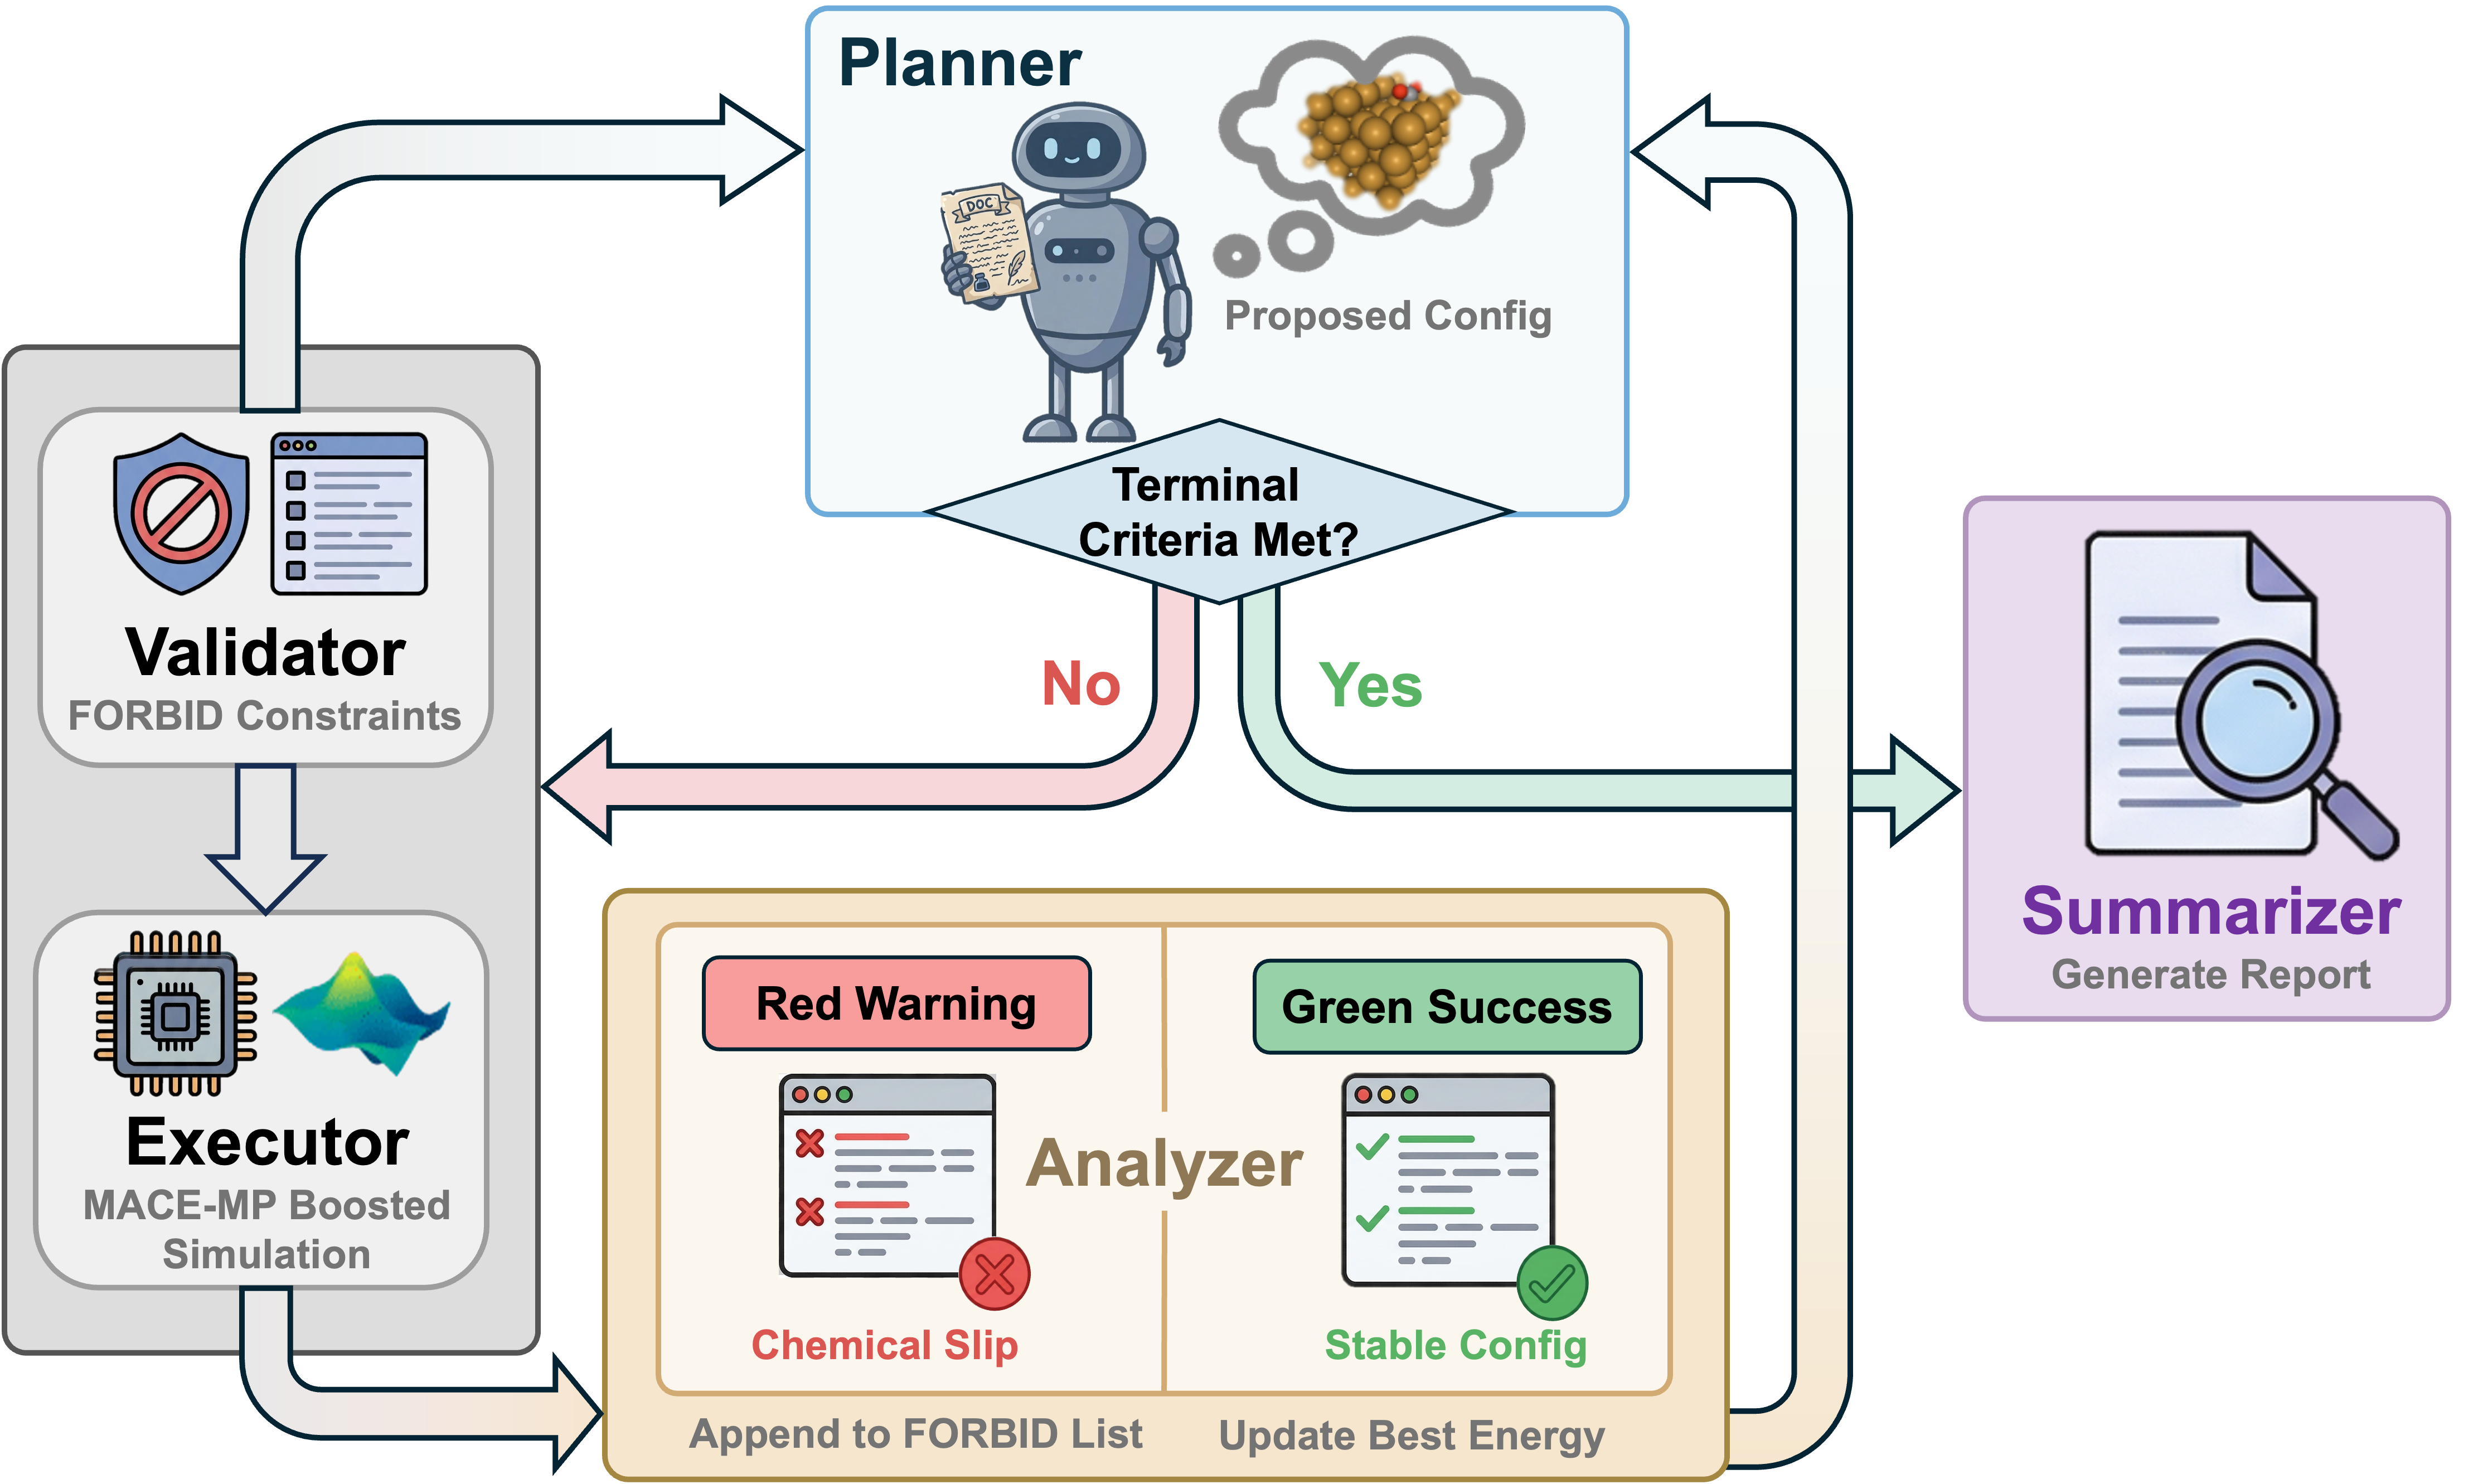
\includegraphics[width=0.75\linewidth]{images/pipeline.png}
    \caption{\textbf{Overview of AdsMind.} (a) Schematic diagram of the AdsMind closed-loop multi-agent framework, showing the Planner, Validator, Executor, Analyzer, and Summarizer agents. (b) Test benchmark datasets: CMU20 (20 monometallic and intermetallic surfaces) and OCD-GMAE62 (62 oxide, compound, and alloy surfaces across two testing tiers). (c) Real-world application: comparison with DFT calculations on selected cases.}
    \label{fig:pipeline}
\end{figure}
